\chapter{Theoretical Overview}
\label{chap:theory}
This chapter describes the physics backgrounds of this thesis.
%Section~\ref{sec:SM} introduces the Standard Model of the particle physics.

\section{The Standard Model}
\label{sec:SM}

The Standard Model (SM) represents a description of the elementary particles and their interactions.
It is a successful theory model to explain the experimental results until today, and it has predicted a lot of parameters e.g. top-quark and higgs-boson masses.
All particles predicted by SM has been confirmed, most recently the Higgs boson was discovered by ATLAS and CMS in 2012.
The SM predicts the existence of elementary particles which form the matter, fermions, consisting of leptons and quarks.
The interactions of them are described by gauge fields mediated by the exchange of corresponding gauge bosons.
There are four types of known interactions in nature, namely electromagnetic, weak and strong force, and gravitational interactions.
The first three of them are described by the SM.

The theoretical description is given with the Quantum Field Theory (QFT) framework. 
The invariance under the local gauge transformation is the key of the framework. 
The underlying symmetry described by Lie groups is written by SU(3)$_C \times$ SR(2)$_L \times$ U(1)$_Y$ gauge group, and some more details are discussed in the following subsections. 

\subsection{Particle Content}
Figure~\ref{fig:SM} shows 17 fundamental particles, consisting of the SM.
\begin{figure}[tbp]
\begin{center}
%\subfigure[]{
 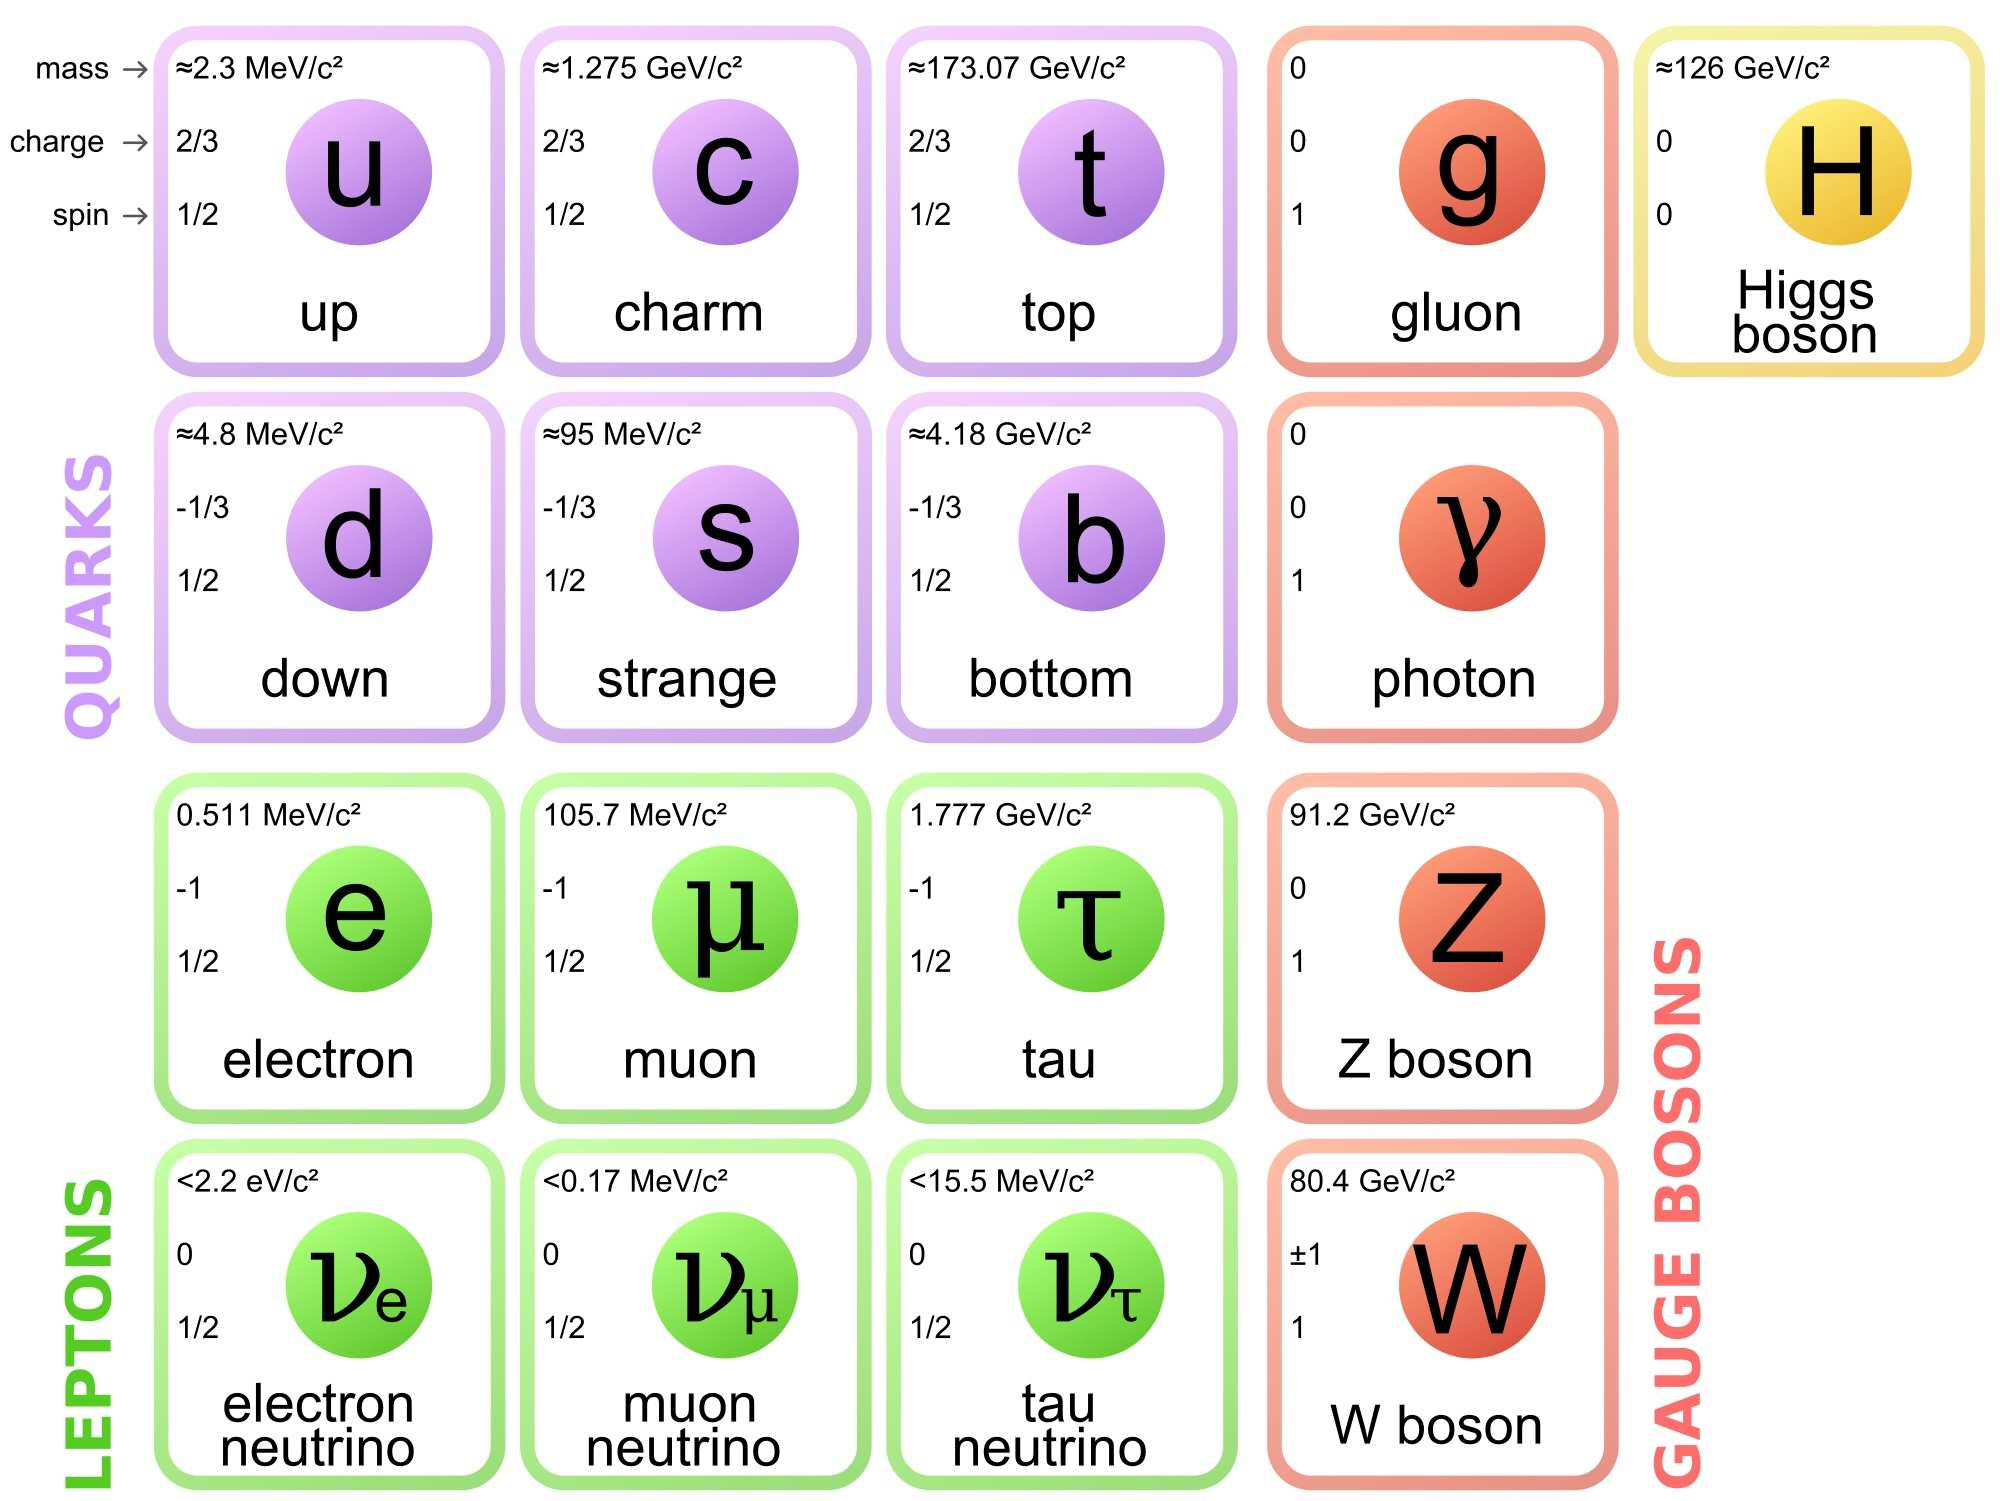
\includegraphics[width=0.85\textwidth,keepaspectratio]{figures/SM}
%}
\caption{
All particles exist in the SM %\ref{}
}
\label{fig:SM}
\end{center}
\end{figure}

They are classified into two types following Fermi-Dirac or Bose-Einstein statistics.
\begin{itemize}
    \item Fermion \\
    Fermions are the elementary particles with spin 1/2. There have three generations also known as flavors.  The particle mass is increased from first to the third generations. The other parameters are exactly the same for those in the same category. They are two types of fermions, quarks and leptons, each has 6 particles. Quark has up-type and down-type quark and lepton has charged and neutral lepton, classified by its charge. Leptons do not act through the strong force, unlike the quarks.
    \item Boson \\
    Bosons are integer-spin particles and mediate the interaction of the fermions.
    The photon ($\gamma$) is the mediator of the electromagnetic force. The photon is massless and stable, hence the electromagnetic force can reach infinite ranges. 
    The photons interact with every particles with electric charges.
    The gluon (g) is the intermediate particle of the strong force. The gluon is also massless, and interact with particles with the color charge, i.e. quarks.
    In addition, due to the non-Abelian nature of the SU(3) gauge group, gluons have a self coupling and they can interact with each other.
    The W$^\pm$ and the Z bosons carry the weak force. They are massive particles and interact with all particles carrying the weak hyper charges. The W$^\pm$ can change the flavor of the quarks. 
\end{itemize}

\subsection{SM Lagrangian}
\label{subsec:Lagrangian}
The SM Lagrangian and its origin are shown in this subsection. 
They are mathematically described as the Lagrangian density, $\mathcal{L}$, and hereafter it is denoted as Lagrangian.\\

\noindent\textbf{\sf{Quantum Electro Dynamics (QED)}} \\ 
The QED describes the dynamics of fermions and their electromagnetic interactions.

The free fermion with the spin 1/2 is described by the Lagrangian\\
\begin{equation}
\label{eqn:QED}
\mathcal{L}=i \bar{\psi} \gamma^{\mu} \partial_{\mu} \psi-m \bar{\psi} \psi
\end{equation}
The $\psi$ here is the spinor of the fermion field, $\gamma^{\mu}$  ($\mu$ = 0,1,2,3) is the Dirac gamma 4$\times$4 matrix. $\partial_{\mu}$ = $\frac{\delta}{\delta x_{\mu}}$ are the partial derivatives, and the $\bar{\psi}=\psi^{\dagger} \gamma^{0}$.
Solving the lagrangian equation fo this yields, the Dirac equation of motion for $\psi$:
\begin{equation}
\left(i \gamma^{\mu} \partial_{\mu}-m\right) \psi=0
\end{equation}
The Lagrangian needs to be invariant under the "local" gauge transformation, i.e. the guage transformation parameter depends on x:
\begin{equation}
\psi(x) \rightarrow \psi^{\prime}(x)=e^{i \alpha(x)} \psi(x)
\end{equation}
where the local phase is given by $\alpha(x)$, depending on space and time. 
This transformation form the Abelian unitary group U(1) with e$^{i\alpha(x)}$ written as the 1$\times$1 matrix with $U^{\dagger} U=1$.
The first term of the Lagrangian (\ref{eqn:QED}) is not invariant under this transformation:
\begin{equation}
\partial_{\mu} \psi \rightarrow \partial_{\mu} \psi^{\prime}=e^{i \alpha(x)} \partial_{\mu} \psi+i e^{i \alpha(x)} \psi \partial_{\mu} \alpha(x)
\end{equation}
The requirement of the invariance leads to introduce an additional field A$_\mu$, transforming as:
\begin{equation}
A_{\mu} \rightarrow A_{\mu}^{\prime}=A_{\mu}+\frac{1}{e} \partial_{\mu} \alpha(x)
\end{equation}
where e is a coupling constant, which is the elementary electric charge 
and $\partial_{\mu}$ is replaced with the covariant derivative D$_\mu$:
\begin{equation}
D_{\mu}=\partial_{\mu}-i e A_{\mu}
\end{equation}
Then the derivative part can be replaced with:
\begin{equation}
D_{\mu} \psi \rightarrow D_{\mu}^{\prime} \psi^{\prime}=e^{i \alpha(x)} D_{\mu} \psi
\end{equation}
which leads the Lagrangian as:
\begin{equation}
\begin{aligned}
\mathcal{L} &=i \bar{\psi} \gamma^{\mu} D_{\mu} \psi-m \bar{\psi} \psi \\
&=\bar{\psi}\left(i \gamma^{\mu} \partial_{\mu}-m\right) \psi+e \bar{\psi} \gamma^{\mu} \psi A_{\mu}
\end{aligned}
\end{equation}
The Lagrangian now restores the invariance with the gauge field A$_\mu$. By using the strength tensor $F_{\mu \nu}=\partial_{\mu} A_{\nu}-\partial_{\nu} A_{\mu}$, the Lagrangian of QED is defined as:
\begin{equation}
\label{eqn:QEDLagrangian}
\mathcal{L}_{\mathrm{QED}}=i \bar{\psi} \gamma^{\mu} \partial_{\mu} \psi-m \bar{\psi} \psi+e \bar{\psi} \gamma^{\mu} \psi A_{\mu}-\frac{1}{4} F_{\mu \nu} F^{\mu \nu}
\end{equation}
The Lagrangian is invariant under the U(1)$_{EM}$ local gauge transformations of fields. The field A$_\mu$ is identified as photon, and the invariance forbids the introduction of a mass term of the A$_\mu$, of the form of $\frac{1}{2}m^2 A_\mu A^\mu$. The photon is requested to be massless, which agrees with all experiment results.
\\

\noindent\textbf{\sf{Quantum Chromo Dynamis (QCD)}} \\ 
The QCD describes the strong force interactions between quarks and gluons. The concept of the required invariance is similar to the QED, while an additional degree of freedom is introduced: the charge denoted as color, red (r), green(g), and blue(b). 
The Dirac spinor is replaced with vector of three spinors for quarks:
\begin{equation}
\psi=\left(\begin{array}{c}
\psi_{r} \\
\psi_{g} \\
\psi_{b}
\end{array}\right)
\end{equation}
The Lagrangian of QCD is described as:
\begin{equation}
\mathcal{L}_{\mathrm{QCD}}=i \bar{\psi} \gamma^{\mu} \partial_{\mu} \psi-m \bar{\psi} \psi-g_{s}\left(\bar{\psi} \gamma^{\mu} \frac{\lambda_{a}}{2} \psi\right) G_{\mu}^{a}-\frac{1}{4} G_{\mu \nu}^{a} G_{a}^{\mu \nu}
\end{equation}
with the gauge fields $G_{\mu}^{a}$ (a = 1,2,...,8) represents the gluons.
While QED is an Abelian gauge theory, for QCD, the underlying group is the non-Abelian group SU(3)$_C$, whose generators are T$_a$ = $\lambda_{a}/2$. $\lambda_{a}$ are callsed Gell-Mann matrices. They satisfy the commutator relation:
\begin{equation}
\left[\frac{\lambda_{a}}{2}, \frac{\lambda_{b}}{2}\right]=i f_{a b c} \frac{\lambda_{c}}{2}
\end{equation}
g$_s$ denotes the strong coupling constatnt, and $G_{a}^{\mu \nu}$ is the field strength tensor, written as:
\begin{equation}
G_{\mu \nu}^{a}=\partial_{\mu} G_{\nu}^{a}-\partial_{\nu} G_{\mu}^{a}-g_{s} f_{a b c} G_{\mu}^{b} G_{\nu}^{c}
\end{equation}
The non-Abelian group structure produces the last term of the field strength, which enables the gluons to interact with themselves differently from QED. Gluons are also requested to be massless from the gauge transformation of the fields.
%quark 
%asymptotic freedom 

\\ \\

\noindent\textbf{\sf{ElectroWeak Model}} \\
It is shown by experiments that the weak interaction only acts on left-handed fermions. In the electroweak model, the SU(2)$_L \times$ U(1)$_Y$ symmetry is conserved. Here the left-handed fermions are assigned to SU(2)$_L$ doublets with weak isospin I = 1/2, and gauge field W$^a_\mu$. The right-handed fermions are assigned to  U(1)$_Y$ singlets with weak isospin I = 0, and gauge field B$_\mu$.
%table of the quantum numbers
The left-handed doublets and right-handed singlets are denoted as $\chi_{L}$ and $\psi_{R}$ ,respectively. Specifically $\chi_{L}$ is written as 
$
\left(\begin{array}{c}
\nu_{L} \\
e_{L}
\end{array}\right)
$
for the leptons of the first generation, and $\psi_{R}$ is written as $(e_R)$.
For the quarks of the first generation, $\chi_{L}$ is 
$
\left(\begin{array}{c}
u_{L} \\
d_{L}
\end{array}\right)
$
and $\psi_{R}$ is $(u_R)$ and $(d_R)$.




These behave under the local gauge transformations as:
\begin{equation}
\begin{aligned}
\chi_{L}(x) \rightarrow \chi_{L}^{\prime}(x) &=e^{i \alpha_{a}(x) \tau_{a}} e^{i \beta(x) Y} \chi_{L} \\
\psi_{R}(x) \rightarrow \psi_{R}^{\prime}(x) &=e^{i \beta(x) Y} \psi_{R}
\end{aligned}
\end{equation}
where $\alpha_{a}(x)$ and $\beta(x)$ are the local phases, $\tau_{a}$ are the generators of SU(2)$_L$ with a = 1,2,3, and Y is the weak hypercharge operator of U(1)$_Y$. The covariant derivative is:
\begin{equation}
D_{\mu}=\partial_{\mu}+i g W_{\mu}^{a} \frac{\tau_{a}}{2}+i g^{\prime} B_{\mu} \frac{Y}{2}
\end{equation}
g here is the coupling constant of the SU(2)$_L$ gauge field written as $W_{\mu}^{a}$. $g^{\prime}$ is the coupling constant of the U(1)$_Y$ gauge field $B_{\mu}$.
The electroweak Lagrangian results in:
\begin{equation}
\mathcal{L}_{\mathrm{EW}}=i \overline{\chi_{L}^{i}} \gamma^{\mu} D_{\mu} \chi_{L}^{i}+i \overline{\psi_{R}^{i}} \gamma^{\mu} D_{\mu} \psi_{R}^{i}-\frac{1}{4} W_{\mu \nu}^{a} W_{a}^{\mu \nu}-\frac{1}{4} B_{\mu \nu} B^{\mu \nu}
\end{equation}
The field strength tensors are:
\begin{equation}
\begin{aligned}
W_{\mu \nu}^{a} &=\partial_{\mu} W_{\nu}^{a}-\partial_{\nu} W_{\mu}^{a}-g \epsilon_{a b c} W_{\mu}^{b} W_{\nu}^{c} \\
B_{\mu \nu} &=\partial_{\mu} B_{\nu}-\partial_{\nu} B_{\mu}
\end{aligned}
\end{equation}
where $\epsilon_{a b c}$ is an antisymmetric tensor, which is the structure constant of SU(2)$_L$. This term enables the $W_{a}^{\mu \nu}$ field to interact with themselves, while $B_{\mu}$ cannot self-interact.
The physical fields represents the W$^{\pm}$, Z bosons and photons are formed by linear combination of $W_{\mu \nu}^{a}$ and $B_{\mu \nu}$.
\begin{equation}
\begin{aligned}
W_{\mu}^{\pm} &=\frac{1}{\sqrt{2}}\left(W_{\mu}^{1} \mp i W_{\mu}^{2}\right) \\
Z_{\mu} &=\cos \theta_{W} W_{\mu}^{3}-\sin \theta_{W} B_{\mu} \\
A_{\mu} &=\sin \theta_{W} W_{\mu}^{3}+\cos \theta_{W} B_{\mu}
\end{aligned}
\end{equation}
where the $\theta_{W}$ = arctan ( g$^{\prime}$/g) represents the weak mixing angle, so called Weinberg angle. By rewriting the Lagrangian with physical fields and comparing the comparing the $A_{\mu}$ components with the QED Lagrangian (\ref{eqn:QEDLagrangian}), the relations between e and g, g$^{\prime}$ is obtained:
\begin{equation}
\begin{aligned}
e&=g \sin \theta_{W}=g^{\prime} \cos \theta_{W} \\
and \ \ Q&=I_{3}+\frac{Y}{2}
\end{aligned}
\end{equation}
The local gauge invariance forbids the introduction of the mass term of the bosons like $m^2_W W_\mu W^\mu$, since it is not invariant under $SU(2)_L \times U(1)_Y$ local transformations.
This statement that the local phase invariance in the electroweak model requests the fermions and bosons to be massless particles, is conflicted against the experimental results, where W$^{\pm}$ , Z bosons and fermions are found to be massive.
\\ \\
\noindent\textbf{\sf{Spontaneously Symmetry breaking}} \\ 
The disagreement of the electroweak model forbidding the masses of the fermions and bosons with the experimental results can be solved by introducing a spontaneously symmetry breaking.
It is known as Brout-Englert-Higgs (BEH) mechanism or “Higgs mechanism” for short.

A complex scalar field, $\phi$, which is a weak isospin doublet, with four degrees of freedom is introduced as the Higgs field:
\begin{equation}
\label{eqn:higgsphi}
\phi=\left(\begin{array}{l}
\phi^{+} \\
\phi^{0}
\end{array}\right)=\frac{1}{\sqrt{2}}\left(\begin{array}{l}
\phi_{1}+i \phi_{2} \\
\phi_{3}+i \phi_{4}
\end{array}\right)
\end{equation}
The corresponding Lagrangian is written as:
\begin{equation}
\label{eqn:Higgs}
\mathcal{L}_{\text {Higgs }}=\left(D_{\mu} \phi\right)^{\dagger}\left(D^{\mu} \phi\right)-\mu^{2} \phi^{\dagger} \phi-\lambda\left(\phi^{\dagger} \phi\right)^{2}
\end{equation}
This is invariant under SU(2)$_l$ $\times$ U(1)$_Y$ phase transformation.
The potential of $\phi$ can be parametrize as:
\begin{equation}
V(\phi)=\mu^{2} \phi^{\dagger} \phi+\lambda\left(\phi^{\dagger} \phi\right)^{2}
\end{equation}
where $\lambda$ > 0. The value of the $\Phi$ at the vacuum is chosen by minimizing $V(\Phi)$. 
In case $-\mu^{2}>0$, the $V(\Phi)$ has its minimum value at 
\begin{equation}
\label{eqn:vacuum}
\phi_{0}&=\frac{1}{\sqrt{2}}\left(\begin{array}{l}
0 \\
v
\end{array}\right)
\end{equation}
where $v = \sqrt {-\mu^{2}/\lambda}$, while in case $-\mu^{2}<0, \phi_{0}=0$ gives the minimum of $V(\phi)$. 
The $v$ is called vacuum expectation value. In the former case, by assigning the ground state of the equation~\ref{eqn:vacuum} the local $SU(2)_L \times U(1)_Y$ symmetry of the vacuum is broken spontaneously. 
Three of the four degrees of freedom of the gauge field (\ref{eqn:higgsphi}) are absorbed by the $W^\pm$ and Z bosons, and the fourth generates the Higgs boson.

%The $\Phi(x)$ can be expanded near its minimum;
%\begin{equation}
%\phi=\frac{1}{\sqrt{2}} \exp \left(\frac{i}{2} \tau_{i} \chi^{\prime %i}(x)\right)\left(\begin{array}{c}
%0 \\
%v+h(x)
%\end{array}\right)
%\end{equation}
%where h(x) represents the Higgs Boson associated to the Higgs fields. The exponential containing  %$\chi^{\prime i}$ (x = 1,2,3) fields (GoldStone Boson) has three degrees of freedom. The local phase %invariance define a specific $\Phi$ as:
%\begin{equation}
%\phi=\frac{1}{\sqrt{2}}\left(\begin{array}{c}
%0 \\
%v+h(x)
%\end{array}\right)
%\end{equation}
%so compare to the equation ref{eqn:eqn:higgsphi}, $\phi_{1}=\phi_{2}=\phi_{4}=0$ and $\phi_{3} = v + %h(x)$. 

The field is parameterized as:
\begin{equation}
\phi(x)=\frac{e^{i \tau_{a} \theta_{a}(x) / v}}{\sqrt{2}}\left(\begin{array}{c}
0 \\
v+h(x)
\end{array}\right)
\end{equation}
where $\theta_{a}(x)$ (a = 1,2,3) and $h(x)$ are the real field, and  $h(x)$ represents the Higgs boson which associated to the Higgs fields. The exponential term including $\theta_{a}(x)$ is defined to be specifical since local gauge transformation needs to be invariant;
\begin{equation}
\phi=\frac{1}{\sqrt{2}}\left(\begin{array}{c}
0 \\
v+h(x)
\end{array}\right)
\end{equation}
The specific gauge has been chosen by defining the vacuum expectation value. That is why we call spontaneously symmetry breaking. 

The Lagrangian of Higgs (\ref{eqn:Higgs}) can be substituted and 
%%*****************************************
%\begin{equation}
%\left|\left(\partial_{\mu}+i g W_{\mu}^{a} \frac{\tau_{a}}{2}+i g^{\prime} B_{\mu} \frac{Y}{2} %\right) \frac{1}{\sqrt{2}}\left(\begin{array}{l}
%0 \\
%v
%\end{array}\right) \right| -\mu^{2} \Phi^{\dagger} \Phi-\lambda\left(\Phi^{\dagger} %\Phi\right)^{2}
%\end{equation}
%%*****************************************
the terms represent the mass terms and its relations are written as:
\begin{equation}
\begin{aligned}
\left|\left(i g \frac{\tau_{a}}{2} W_{\mu}^{a}+i g^{\prime} \frac{Y}{2} B_{\mu}\right) \phi_{0}\right|=&\left(\frac{1}{2} v g\right)^{2} W_{\mu}^{+} W^{\mu-} \\
&+\left(\frac{1}{2} v g\right)^{2} \frac{1}{2 \cos ^{2} \theta_{W}} Z_{\mu} Z^{\mu} \\
&+0 \cdot A_{\mu} A^{\mu}
\end{aligned}
\end{equation}
%%Calculate this!
%which the mass terms of the vector bosons can be written:
%\begin{equation}
%\begin{aligned}
%m_{W}&=\frac{1}{2} vg \\
%m_{Z}&=\frac{m_{W}}{\cos \theta_{W}} \\
%m_{\gamma}&=0
%\end{aligned}
%\end{equation}
The mass terms for the $W_\pm$ and Z bosons naturally obtained through the symmetry breaking of SU(2)$_L$. :
\begin{equation}
\begin{aligned}
m_{\gamma} &=m_{A}=0 \\
m_{Z} &=\frac{v}{2} \sqrt{g^{2}+g^{\prime 2}} \\
m_{W} &=\frac{v}{2} g
\end{aligned}
\end{equation}

%The $A_\mu$ does not acquire the mass term, as the photons are remained to be massless.
%There is a term $-\mu_{\phi}^{2} h^{2}=\lambda v^{2} h^{2}$ and from this term the Higgs boson %gains mass itself, which leads to the Higgs boson mass 
%\begin{equation}
%m_{H}=\sqrt{-2 \mu^{2}}=\sqrt{2 \lambda} v
%\end{equation}
%The parameter $\lambda$ is a free parameter in the theory, so it cannot be predicted by the SM.
%The vacuum expectation value is is determined by the measurements of the Fermi constant $G_F$, %which is to be:
%%put reference here (measurement of the Fermi coupling) 
%\begin{equation}
%v=\frac{2 m_{W}}{g}=\frac{1}{\sqrt{2} G_{F}} \simeq 246.22 \mathrm{GeV}
%\end{equation}

\\ \\
\noindent\textbf{\sf{Yukawa Coupling}} \\ 
The fermion mass term is also not invariant under the local phase transformations of SU(2)$_L$. It is also generated with the Higgs mechanism, using their coupling to the Higgs boson. The newly introduced coupling $g_f$ is called Yukawa coupling.

For the down type fermions, the same Higgs field $\phi$ is used, while for the up type fermions, the charge conjugate of the Higgs field $\phi^C$ is employed instead:
\begin{equation}
\phi^{c}=i \tau_{2} \phi^{*}=\left(\begin{array}{c}
\phi^{0 *} \\
-\phi^{+*}
\end{array}\right)
\end{equation}
For the quarks, the additional Lagrangian can be described as follows:
\begin{equation}
\mathcal{L}_{q}=\left[-g_{d}\left(\bar{\psi}_{L}^{d} \phi \psi_{R}^{d}\right)+\text { h.c. }\right]+\left[-g_{u}\left(\bar{\psi}_{L}^{u} \phi^{c} \psi_{R}^{u}\right)+\text { h.c. }\right]
\end{equation}
These are local gauge invariant before the symmetry breaking. After the symmetry breaking, $\phi^C$ can be written as:
\begin{equation}
\phi^{c} 
%\rightarrow 
=\frac{1}{\sqrt{2}}\left(\begin{array}{c}
v+h \\
0
\end{array}\right)
\end{equation}
Then the additional Lagrangian substituted into:
\begin{equation}
\mathcal{L}_{q}=-\frac{1}{\sqrt{2}} g_{d} v \bar{d}_{L} d_{R}\left(1+\frac{h}{v}\right)-\frac{1}{\sqrt{2}} g_{u} v \bar{u}_{L} u_{R}\left(1+\frac{h}{v}\right)
\end{equation}
In case of leptons the additional Lagrangian is:
\begin{equation}
\mathcal{L}_{e}=\left[-g_{e}\left(\bar{\psi}_{L}^{e} \phi \psi_{R}^{e}\right)+\text { h.c. }\right]
\end{equation}
then after the symmetry breaking:
\begin{equation}
\mathcal{L}_{e}=-\frac{1}{\sqrt{2}} g_{e} v \bar{e}_{L} e_{R}\left(1+\frac{h}{v}\right)
\end{equation}

The mass of the fermions is to be obtained as:
\begin{equation}
m_{f}=\frac{1}{\sqrt{2}} g_{f} v
\end{equation}

When summarizing the quarks and leptons, Lagrangian of the Yukawa couplings can be written as:
\begin{equation}
\mathcal{L}_{\text {Yukawa }}=-g_{l}^{i j} \bar{\Psi}_{L}^{i} \phi l_{R}^{j}-g_{d}^{i j} \bar{\Psi}_{L}^{i} \phi d_{R}^{j}-g_{u}^{i j} \bar{\Psi}_{L}^{i} \phi^{C} u_{R}^{j}+\text { h.c. }
%?? is this correct ??
\end{equation}

Finally, the total Standard Model Lagrangian is described as 
\begin{equation}
\mathcal{L}_{\mathrm{SM}}=\mathcal{L}_{\mathrm{QCD}}+\mathcal{L}_{\mathrm{EW}}+\mathcal{L}_{\text {Higgs }}+\mathcal{L}_{\text {Yukawa}}
\end{equation}
This Lagrangian is invariant under local transformations of SU(3) $\times$ SU(2)$_L$ $\times$ U(1)$_Y$, while the vacuum is breaking the symmetry and not invariant. \\

The coupling constants appeared in the Lagrangian are determined by the experimental measurement. 
The measured values are summarized in the Table~\ref{tab:constants}.  \\

\begin{center}
\begin{table}
\centering
\begin{tabular}{|c|c|}
\hline
Coupling constants & Measured Value \\
\hline 
                             & $y_{u}=10^{-5}, y_{c}=7 \times 10^{-5}, y_{t}=1,$, \\
            Yukawa Couplings & $y_{d}=3 \times 10^{-5}, y_{s}=5 \times 10^{-4}, y_{b}=0.03$ \\
                             & $y_{e}=3 \times 10^{-6}, y_{\mu}=6 \times 10^{-4}, y_{\tau}=0.01$ \\
     Fine Structure Constant & $\alpha=1 / 127$ \\
    Strong Coupling Constant & $\alpha_{s}=0.12$ \\
              Weinberg Angle & $s_{W}^{2}=0.23$ \\
Higgs Self Coupling Constant & $\lambda=0.1$ \\
%PMNS matrix (parametric representation) & $\theta_{12}=34, \theta_{13}=8.5, \theta_{23}=247, \delta_{C P}=200$ \\
%CKM matrix (parametric representation) & $\theta_{12}=13.0, \theta_{13}=0.2, \theta_{23}=2.4, \delta_{13}=1.2$ \\
\hline
\end{tabular}
\caption{coupling constants~\cite{PhysRevD.98.030001}}
\label{tab:constants}
\end{table}
\end{center}

\section{Phenomenology of proton-proton collision}
The standard model physics can be tested with the scattering experiments like pp collisions at LHC.
The physics related to the proton-proton interaction is described in this section. 
%Using the protons instead of the electrons is its higher mass, which enables to reach the higher center-of-mass energy in spite of the energy loss due to the syncrotoron radiation, which is propotional to $m^{-4}$.
Since there is a substructure inside the proton, the proton-proton collision cross section needs to be modeled through the formalism of QCD.

\subsection{Factorization}
\label{subsec:factorization}

The scattering cross section can be calculated with perturbative QCD. 
However, the size of the coupling constant, $\alpha_s$ even at the rather large momentum, $q^2$, the perturbative expansion converges really slow.
The factorization theorem \cite{} allows us to calculate the total cross section approximately with two parts; 
(1) obtaining initial parton that contribute to the hard scattering from the original proton, 
(2) the partonic cross section calculation as illustrated in Figure~\ref{fig:factorization}

\begin{figure}[tbp]
\begin{center}
%\subfigure[]{
 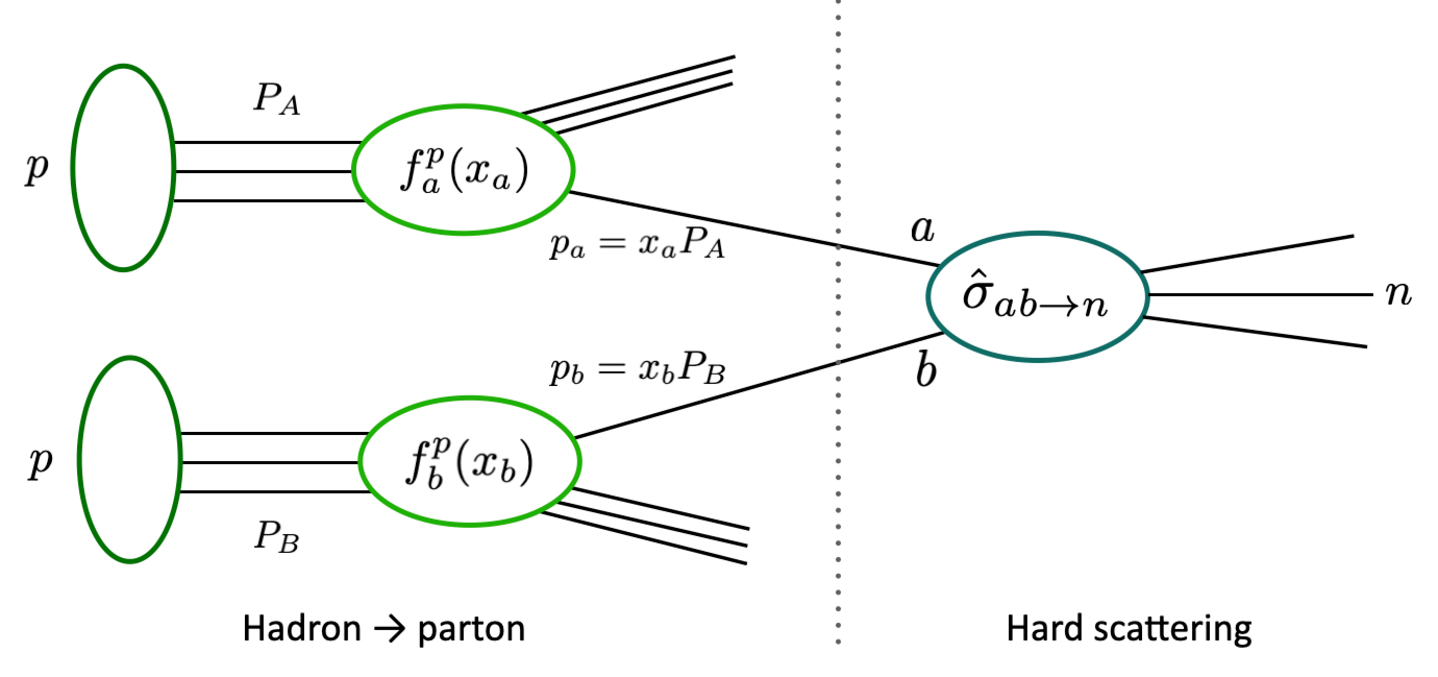
\includegraphics[width=0.8\textwidth,keepaspectratio]{figures/factorization}
%}
\caption{
 factorization theorem 
}
\label{fig:factorization}
\end{center}
\end{figure}

In the scattering process ab$\rightarrow$n at a hadron collider can be written as:
\begin{equation}
\label{eqn:qcdxsec}
\sigma_{a b \rightarrow n}=\sum_{a, b} \int_{0}^{1} \mathrm{~d} x_{a} \mathrm{~d} x_{b} \int \mathrm{d} \Phi_{n} f_{a}^{h_{1}}\left(x_{a}, \mu_{F}\right) f_{b}^{h_{2}}\left(x_{b}, \mu_{F}\right) \times \frac{1}{2 \hat{s}}\left|\mathcal{M}_{a b \rightarrow n}\right|^{2}\left(\Phi_{n} ; \mu_{F}, \mu_{R}\right)
\end{equation}
where a and b is summed over all partonic constituents of the colliding hadrons, $h_1$ and $h_2$, respectively.
$f_{a}^{h_{1}}\left(x_{a}, \mu_{F}\right)$ and $f_{b}^{h_{2}}\left(x_{b}, \mu_{F}\right)$ are the parton distribution function (pdf), obtaining the partons from the original colliding hadrons, at a given momentum fraction x. The factorization depends on the arbitrary cutoff scale, referred as factorization scale, $\mu_F$.
Then the partonic cross section of the hard scattering, $\hat{\sigma}_{a b \rightarrow n}\left(\mu_{F}, \mu_{R}\right)$ can be calculated perturbatively with Feynman-diagrams technique by considering the process $ab\rightarrow n $ with free partons in the initial state. This calculation is done with the Matrix element $\left|\mathcal{M}_{a b \rightarrow n}\right|$ for the phase-space $\Phi_n$.
When calculating the matrix element of the hard-scattering process, the divergence terms are absorbed into the redefinition of fields or parameters via subtractions. This procedure is usually referred as renormalization, and the subtractions scale is called renormalization scale, $\mu_R$. 
The PDF is estimated by the collision data from previous and current experiments, and extrapolated to the appropriate energy using the DGLAP evolution equations.\cite{}.
%this reference can be found in "VBS2014"

Since the matrix-element is calculated at a fixed order, final states of parton-level events calculated so far is neglecting higher-order corrections, which have sizable effect on the particle kinematics. In order to account for effects of higher order QCD correction and hadronization, parton showering and hadronization algorithm are performed.

\subsection{Parton shower}
\label{subsec:partonshower}

The parton shower do the splittings of the outgoing colored partons.  The MC simulations is base on the Markov-chain, in which the components of the hard subprocess are evolved by adding branchings of one parton into two other partons, in the limit of the infrared cutoff scale, t$_{cutoff}$, typically $t_{0} \approx 1 \mathrm{GeV}$. The typical generators: Pythia~\cite{SJOSTRAND2008852} and Herwig~\cite{Gieseke2012} use different choices of t$_{cutoff}$.
The parton shower doesn't affect to the total cross section, since the final state particles emitted to every directions.
\subsection{Hadoronization}
The partons resulted afterparton shower are combined to form hadrons. Hadronization is performed in completely non-pertabative way, based on several models. Phytia and Herwig adopt different phenomenological models: String Model, based on linear confinement of partons and Cluster Model, based on the preconfinement of parton showers.
%\subsection{MC generators}
%description of MC generators, up to where and what they do


\section{Vector Boson Scattering}
\label{sec:VBS}

The scattering of two electroweak vector gauge bosons can probe the structure of the electroweak symmetry breaking (EWSM) mechanism directly. 
The Vector Boson Scattering (VBS) is therefore one of the key process as to be investigated in the LHC experiment.
The Vector Boson indicates W,Z,$\gamma$ here, which are fundamental electroweak bosons. Though the massive vector bosons, which are W and Z are only sensitive to the mechanism of the  EWSM, $\gamma$ is also included since it is impossible to fully separate the $\gamma$ and Z contributions experimentally. 
%<- need this??
%\subsection{Electroweak gauge boson scattering and the Higgs boson}
As described in section~\ref{subsec:Lagrangian}, the spontaneously symmetry breaking of the local gauge invariance with the Higgs field
introduces the masses of the longitudinal, massive weak gauge bosons. 
Measuring the VBS processes provides the information related to that mechanism.
The typical Feynman diagram of VBS is shown in Figure~\ref{fig:VBS}.
%%Correct explanation here????

\begin{figure}[tbp]
\begin{center}
%\subfigure[]{
 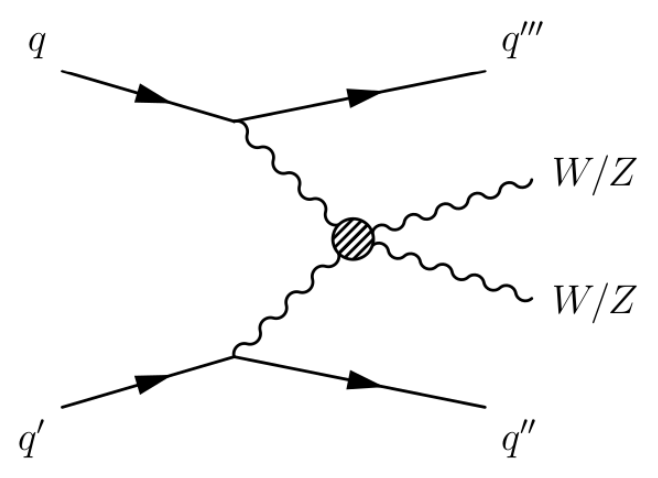
\includegraphics[width=0.50\textwidth,keepaspectratio]{figures/VBS}
%}
\caption{
The Feynman diagram of the VBS. The circle includes any connected diagrams with the external lines at leading order.%, as shown in the Figure\ref{}.
}
\label{fig:VBS}
\end{center}
\end{figure}

\begin{figure}[tbp]
\begin{center}
\subfigure{
 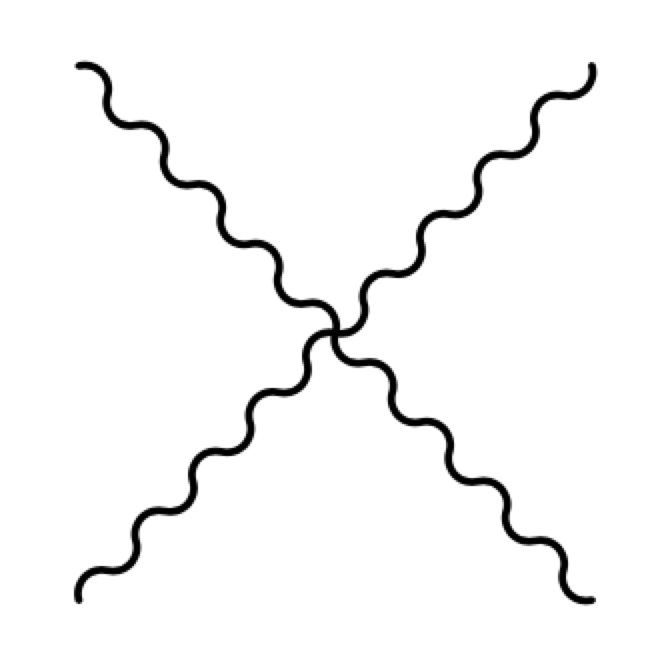
\includegraphics[width=0.20\textwidth,keepaspectratio]{figures/VBS1}
}
\subfigure{
 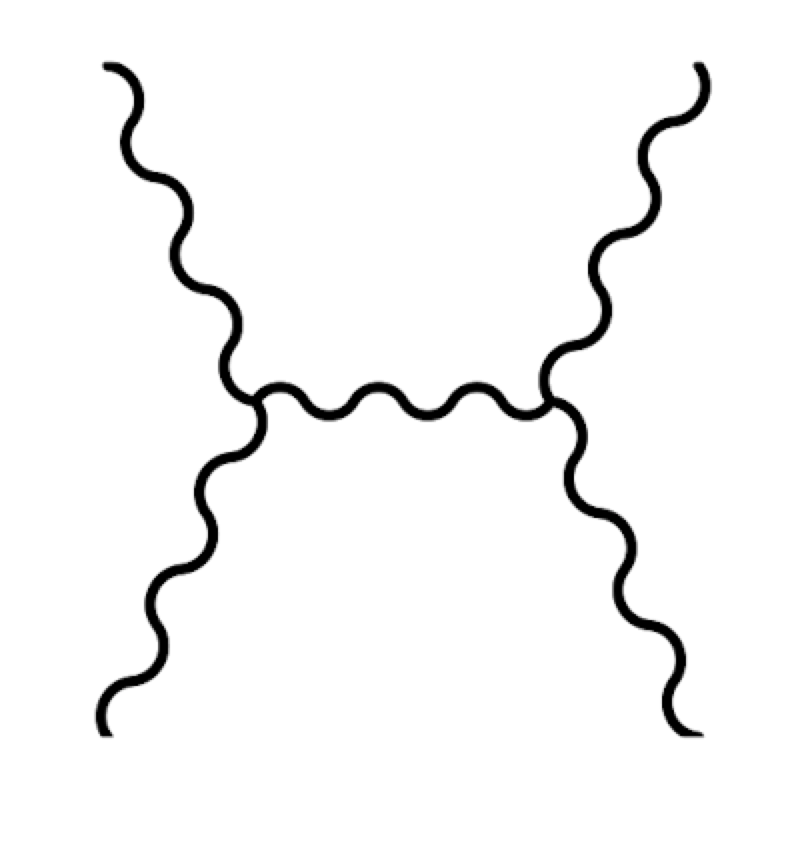
\includegraphics[width=0.19\textwidth,keepaspectratio]{figures/VBS2}
}
\subfigure{
 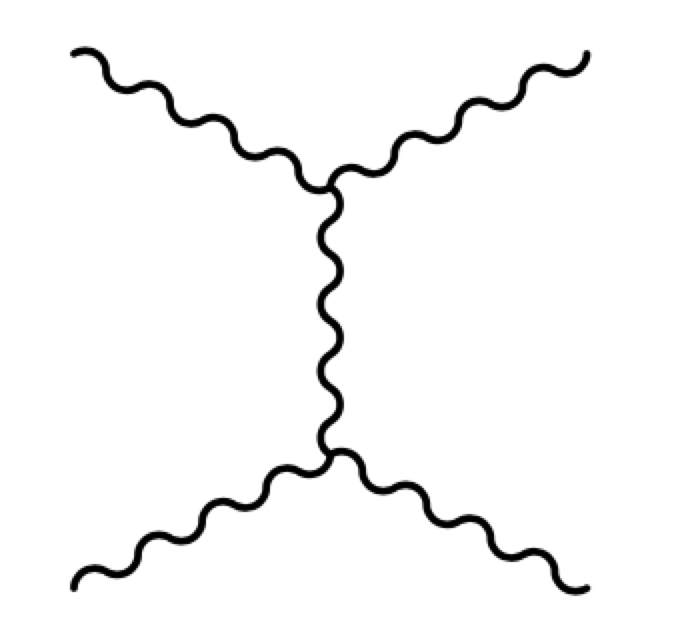
\includegraphics[width=0.21\textwidth,keepaspectratio]{figures/VBS3}
}
\subfigure{
 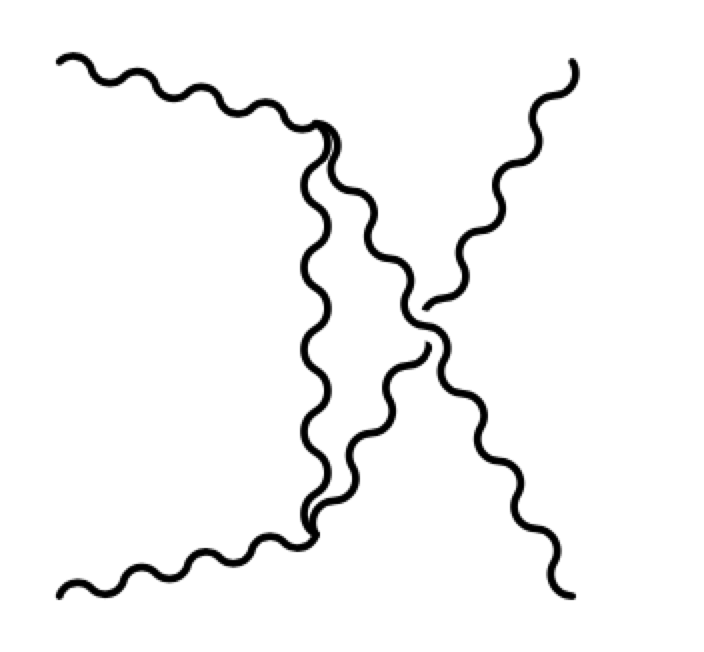
\includegraphics[width=0.21\textwidth,keepaspectratio]{figures/VBS4}
}
\caption{
The VV to VV interaction Feynman diagram at tree-level. Contributions from EW gauge boson interactions.
}
\label{fig:VBSEW}
\end{center}
\end{figure}

\begin{figure}[tbp]
\begin{center}
\subfigure{
 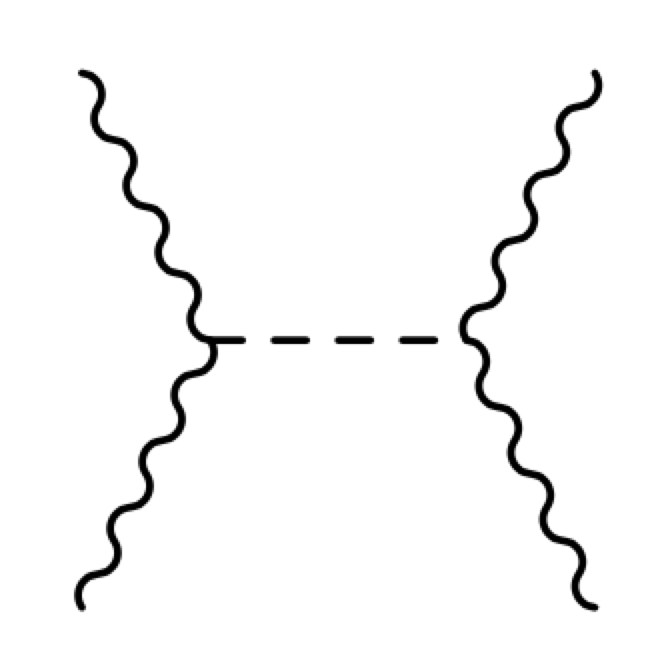
\includegraphics[width=0.20\textwidth,keepaspectratio]{figures/wHiggs1}
}
\subfigure{
 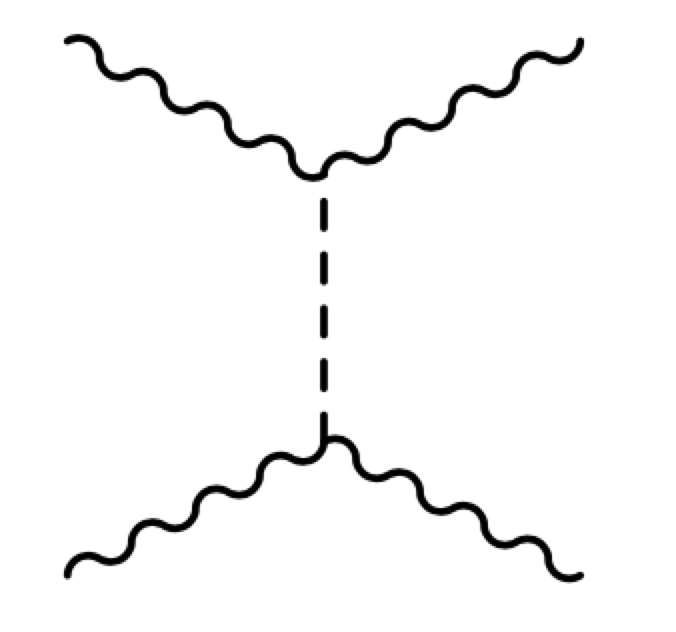
\includegraphics[width=0.20\textwidth,keepaspectratio]{figures/wHiggs2}
}
\subfigure{
 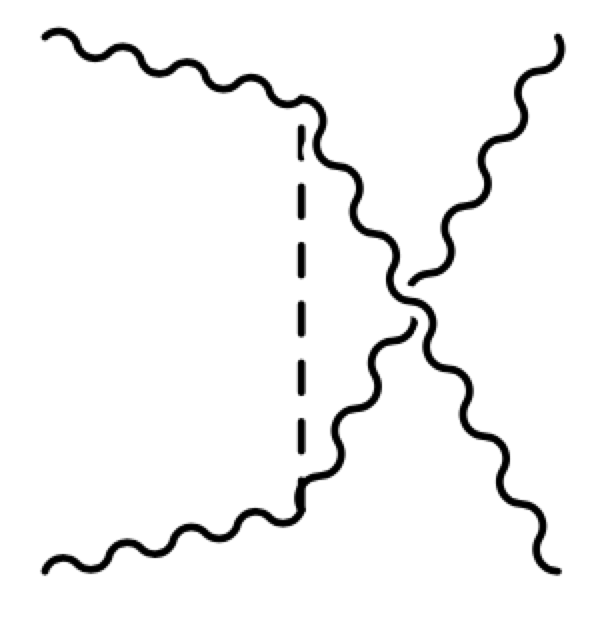
\includegraphics[width=0.18\textwidth,keepaspectratio]{figures/wHiggs3}
}
\caption{
The VV to VV interaction Feynman diagram at tree-level. Contributions includes Higgs boson interactions.
}
\label{fig:VBSHiggs}
\end{center}
\end{figure}


Here, the amplitude of the longitudinal WW scattering is dscussed further to see the effect of existence of the Higgs boson for example. The combination of other weak massive bosons like WZ, as well as ZZ can be denoted similarly. 

Since the polarization vector of the longitudinal weak vector boson can be written in the form, \cite{Rindani_2009}: 
\begin{equation}
\epsilon_{L}^{\mu}=\frac{1}{m_{V}}\left(|\vec{p}|, \frac{\vec{p}}{|\vec{p}|} E\right)=\frac{p^{\mu}}{m_{V}}+\mathcal{O}\left(\frac{m_{V}}{E}\right)
\end{equation}
as the $p_{T}$ glows, the yields with massive vector particles in the initial and finals states will be longitudinal-dominant.
At high-energy limit, the amplitude for $W_L^+W_L^-$ without existing of the Higgs boson (Figure\ref{fig:VBSEW}) can be describes in the form of:
\begin{equation}
\mathcal{M}^{\text {gauge}}=-\frac{g_{w}^{2}}{4 m_{W}^{2}} u+\mathcal{O}\left(\left[\frac{E}{m_{W}}\right]^{0}\right)
\end{equation}
The remaining amplitude from the second term will rise with energy then it violates the unitarity at the unitarity bound. The amplitude including the Higgs contributions (Figure\ref{fig:VBSHiggs}) is:
\begin{equation}
\begin{aligned}
\mathcal{M}^{\text {Higgs}} &=-\frac{g^{2}}{4 m_{W}^{2}}\left[\frac{\left(s-m_{W}^{2}\right)^{2}}{s-m_{H}^{2}}+\frac{\left(t-m_{W}^{2}\right)^{2}}{t-m_{H}^{2}}\right] \\
& \approx \frac{g^{2}}{4 m_{W}^{2}} u,
\end{aligned}
\end{equation}
in the high-energy limit s >> $m_{H}^{2}$, $m_{W}^{2}$.
Therefore the terms affected by the rising energy cancel and leave the constant term, which is not violating the unitarity.
%The energy scale where the unitarity is violated

This effect also described with the Figure~\ref{fig:violation}.
The figure shows that if diagrams with Higgs contribution is missing, the electroweak couplings becomes strong around $\sqrt{s}$ ∼ 1 TeV, and the unitarity of the $W_LW_L \rightarrow W_LW_L$ process is violated, which means the SM without the Higgs boson is no longer valid above TeV-scale. 

\begin{figure}[tbp]
\begin{center}
%\subfigure[]{
 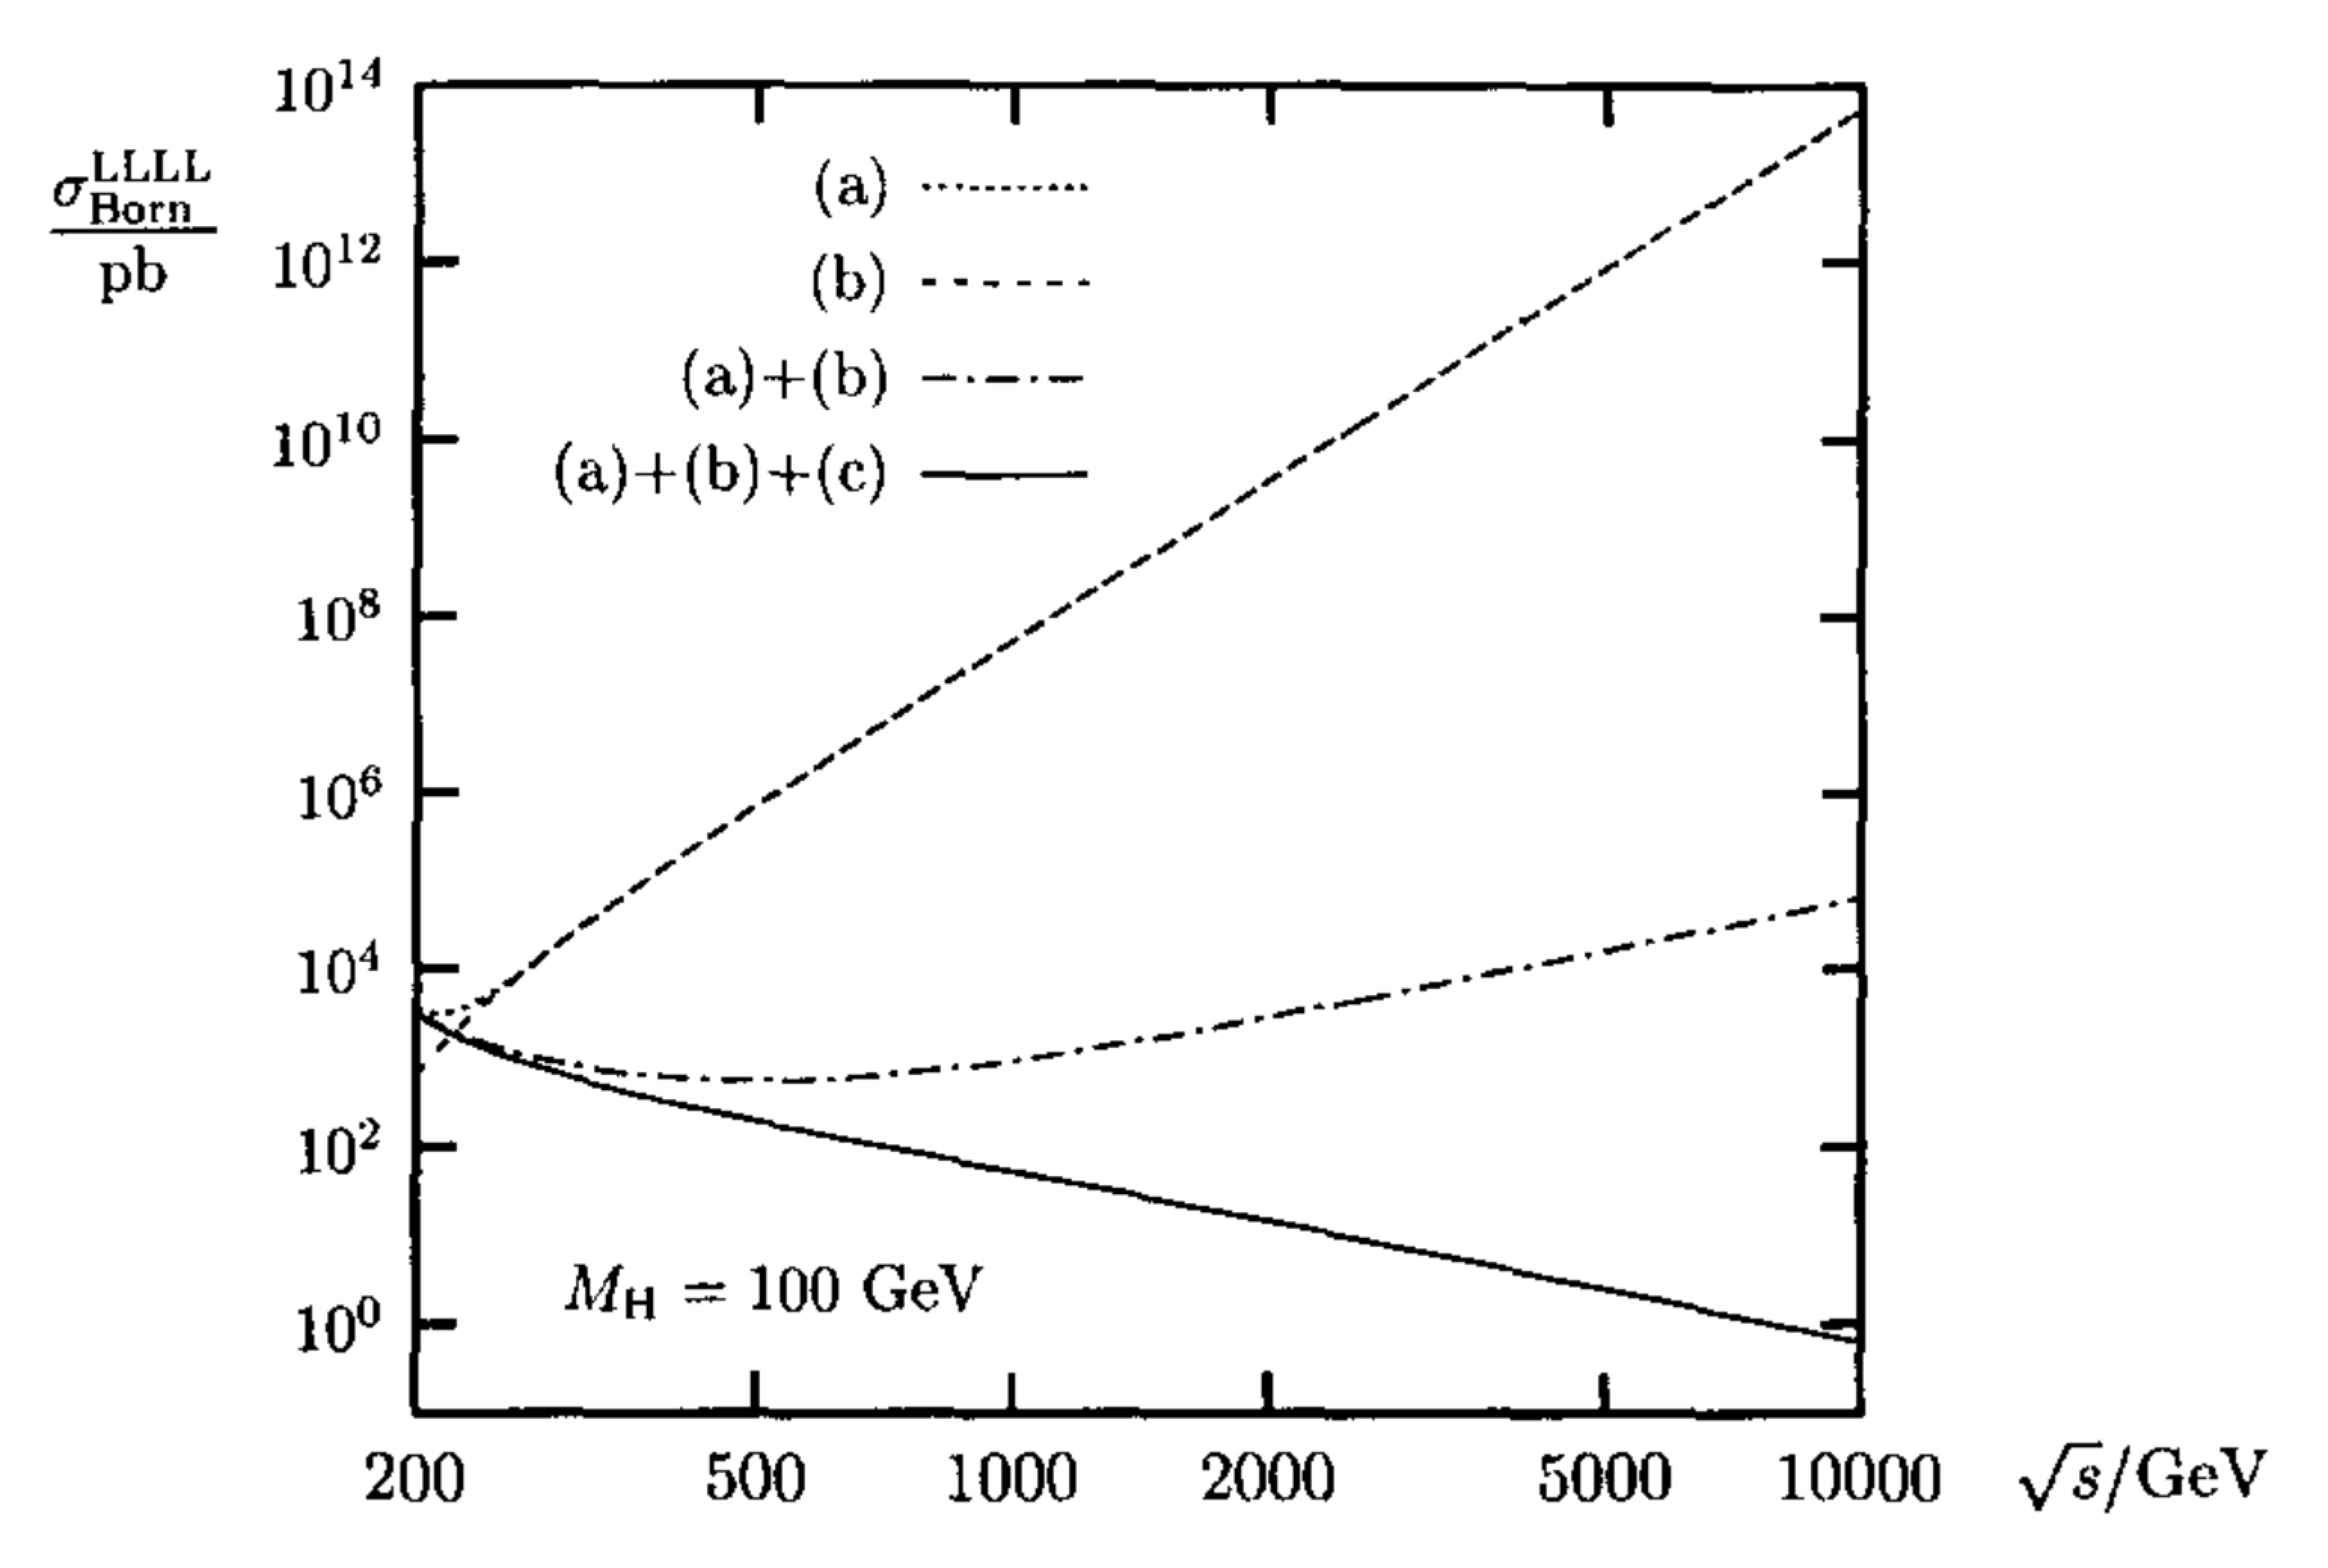
\includegraphics[width=0.80\textwidth,keepaspectratio]{figures/violation}
%}
\caption{
Cross section at tree-level %\ref{}
}
\label{fig:violation}
\end{center}
\end{figure}

%\section{Several decay channels in VBS analysis}
%\section{Experimental results in VBS analysis}
%\textcolor{blue}{put description about the several decay channels and the good point of the semi-leptonic channel here} \\
%There are several decay channels in VBS analysis with respect to the boson type and its decay products. The latest significance obtained by ATLAS and CMS in each channels are summarized in the Table.

%\begin{tabular}{|c|c|c|c|}
%\hline \multicolumn{2}{|c|}{}                                   & ATLAS             & CMS\\
%\hline
%\hline \multirow{3}{*}{ Full-leptonic }      & ssWW -> Ivlv     & $6.5      \sigma$ &    \\
%\cline { 2 - 4 }                             & osWW             & $-$               &    \\
%\cline { 2 - 4 }                             & WZ -> Ivll       & $5.3(3.2) \sigma$ &    \\
%\cline { 2 - 4 }                             & ZZ -> IIll/llvv  & $5.5(4.3) \sigma$ &    \\
%\hline \multicolumn{2}{|c|}{ Semi-leptonic }                    & $2.7(2.5) \sigma$ &    \\
%\hline \multicolumn{2}{|c|}{ Full-hadronic }                    & $-$               &    \\
%\hline
%\end{tabular}

%The VBS process has already observed in the full-leptonic channel.
%In this thesis, semi-leptonic channel is studied. One of the two weak vector boson (W or Z) decay into leptons ( electrons or muons or neutrino) and the other decays into hadrons.

%\textcolor{blue}{put previous analysis results here}

\section{Anomalous Quartic Gauge Coupling and Effective Field Theory}
%\textcolor{blue}{Discuss about dependent models for example compositeness. Then introduce EFT to see them model-independently.} \\
%\subsection{aQGC}
The unitarity recovered by the existence of Higgs boson can be broken again by the additional quartic gauge coupling by new physics. This is referred to as anomalous quartic gauge couplings (aQGC). 

\subsection{EFT}
\label{subsec:EFT}
%Since the aQGC can claim many different models, the Effective Field Theory (EFT) is considered as a model-independent way of the interpretation. 
New physics contribution is generally described by the effective field theory (EFT) as a model-independent way of the interpretation.
The EFT models the effects of new physics at energy scale much higher than the currently accessible range by the experiments. 
%The SM is regarded as an effective theory at low-energy in this framework.
%The EFT contains additional operators with higher energy dimension suppressed by the cutoff scale of the new physics, $\Lambda$.
They are based on the following expansion of the EFT Lagrangian;
\begin{equation}
\label{eq:EFTLagrangian}
\mathcal{L}_{\mathrm{EFT}}=\mathcal{L}_{\mathrm{SM}}+\sum_{d>4} \sum_{i} \frac{f_{i}^{(d)}}{\Lambda^{d-4}} \mathcal{O}_{i}^{(d)}
\end{equation}
where $\Lambda$ is the typical scale of new physics, called cutoff scale. $f_{i}^{(d)}$ are the Wilson coefficients, the dimensionless coupling-strength coefficients of the new operators, $\mathcal{O}_{i}^{(d)}$.
Any new physics can be modeled in this framework by certain additional operators, where their coefficient is also fixed as long as the new physics scale is above $\Lambda$. 
The SM is a low-energy theory in this framework, i.e. if $\Lambda \rightarrow \infty$, the SM is reproduced.
\\
The operators are constructed out of the following fields;
\begin{itemize}
    \item Higgs double field $\Phi$,
    \item covariant derivative $D^{\mu}$,
    \item field strength tensors $W^{\mu\nu}$, $B^{\mu\nu}$,
    \item fermion fields $\psi$
\end{itemize}
In general, all operators with an odd number of dimensions involve fermion fields and lead to lepton or baryon number violation~\cite{PhysRevLett.43.1566}. Therefore we need to consider even dimension only, starting from d = 6.
Equation~\ref{eq:EFTLagrangian} is then written like;
\begin{equation}
\label{eq:EFTLagrangian2}
\mathcal{L}_{\mathrm{EFT}}=\mathcal{L}_{\mathrm{SM}} + \sum_{i} \frac{f_{i}^{(d)}}{\Lambda^{2}} \mathcal{O}_{i}^{(d)} +  \sum_{j} \frac{f_{j}^{(d)}}{\Lambda^{4}} \mathcal{O}_{j}^{(d)} + \cdots
\end{equation}
where the second term represents the dimension-6 operators which affect triple and quartic couplings, and the third term represents the dimension-8 operators, which affect only quartic couplings.
%Numbers of the collider experiments probe triple gauge couplings (TGC) in the pair production of electroweak gauge bosons, while the study of quartic gauge couplings (QGC) requires the production of three electroweak vector bosons, or the VBS of electroweak vector boson pairs. 
%Therefore, the Wilson coeffients of effective operators that contain both TGC and QGC are more strongly constrained through the study of their TGC component, hence most of the present LHC serches for effects of QGC focus on the operators that generate QGC but do not have any TGC associated with them. 
To model possible aQGC effect in the VBS process, the Eboli model \cite{eboli2006p}, introduces new dimension-8 operators which satisfy the SM $SU(2)\times U(1)_Y$ symmetry are used. TGC is already strongly constrained through the study using dimension-6 operators via the pair production of electroweak gauge bosons. To focus more on the effect of QGC, only dimension-8 operators are considered here, as the operators that generate QGC but do no have any TGC associated with them.
%The lowest dimension operator that leads to quartic interactions and does not exhibit two or three weak gauge boson vertices is dimension 8. 
%This is when we get a operator with 
These operators are with weak boson field either from the covariant derivative of Higgs doublet $\Phi$ or from the field strength tensor. 
%In either case the vector field is accompanied by a vacuum expected value or a derivative, therefore the genuine quartic vertices are of dimension 8 or higher.
All the corresponding operators are shown hereafter. The analysis usually focus on these operators on a one-by-one basis.
\begin{itemize}
\item Operators containing just $D_\mu \Phi$ : (Scalor type)
\begin{equation}
\begin{aligned}
\mathcal{O}_{S, 0} &=\left[\left(D_{\mu} \Phi\right)^{\dagger} D_{\nu} \Phi\right] \times\left[\left(D^{\mu} \Phi\right)^{\dagger} D^{\nu} \Phi\right] \\
\mathcal{O}_{S, 1} &=\left[\left(D_{\mu} \Phi\right)^{\dagger} D^{\mu} \Phi\right] \times\left[\left(D_{\nu} \Phi\right)^{\dagger} D^{\nu} \Phi\right] \\
\mathcal{O}_{S, 2} &=\left[\left(D_{\mu} \Phi\right)^{\dagger} D_{\nu} \Phi\right] \times\left[\left(D^{\nu} \Phi\right)^{\dagger} D^{\mu} \Phi\right]
\end{aligned}
\end{equation}
\item Operators containing $D_\mu \Phi$ and field strength : ( Mixed type)
\begin{equation}
\begin{aligned}
\mathcal{O}_{M, 0} &=\operatorname{Tr}\left[\hat{W}_{\mu \nu} \hat{W}^{\mu \nu}\right] \times\left[\left(D_{\beta} \Phi\right)^{\dagger} D^{\beta} \Phi\right] \\
\mathcal{O}_{M, 1} &=\operatorname{Tr}\left[\hat{W}_{\mu \nu} \hat{W}^{\nu \beta}\right] \times\left[\left(D_{\beta} \Phi\right)^{\dagger} D^{\mu} \Phi\right] \\
\mathcal{O}_{M, 2} &=\left[B_{\mu \nu} B^{\mu \nu}\right] \times\left[\left(D_{\beta} \Phi\right)^{\dagger} D^{\beta} \Phi\right] \\
\mathcal{O}_{M, 3} &=\left[B_{\mu \nu} B^{\nu \beta}\right] \times\left[\left(D_{\beta} \Phi\right)^{\dagger} D^{\mu} \Phi\right] \\
\mathcal{O}_{M, 4} &=\left[\left(D_{\mu} \Phi\right)^{\dagger} \hat{W}_{\beta \nu} D^{\mu} \Phi\right] \times B^{\beta \nu} \\
\mathcal{O}_{M, 5} &=\left[\left(D_{\mu} \Phi\right)^{\dagger} \hat{W}_{\beta \nu} D^{\nu} \Phi\right] \times B^{\beta \mu} \\
\mathcal{O}_{M, 6} &=\left[\left(D_{\mu} \Phi\right)^{\dagger} \hat{W}_{\beta \nu} \hat{W}^{\beta \nu} D^{\mu} \Phi\right] \\
\mathcal{O}_{M, 7} &=\left[\left(D_{\mu} \Phi\right)^{\dagger} \hat{W}_{\beta \nu} \hat{W}^{\beta \mu} D^{\nu} \Phi\right]
\end{aligned}
\end{equation}
\item Operators containing just the field strength tensor (Tensor type)
\begin{equation}
\begin{aligned}
\mathcal{O}_{T, 0} &=\operatorname{Tr}\left[\hat{W}_{\mu \nu} \hat{W}^{\mu \nu}\right] \times \operatorname{Tr}\left[\hat{W}_{\alpha \beta} \hat{W}^{\alpha \beta}\right] \\
\mathcal{O}_{T, 1} &=\operatorname{Tr}\left[\hat{W}_{\alpha \nu} \hat{W}^{\mu \beta}\right] \times \operatorname{Tr}\left[\hat{W}_{\mu \beta} \hat{W}^{\alpha \nu}\right] \\
\mathcal{O}_{T, 2} &=\operatorname{Tr}\left[\hat{W}_{\alpha \mu} \hat{W}^{\mu \beta}\right] \times \operatorname{Tr}\left[\hat{W}_{\beta \nu} \hat{W}^{\nu \alpha}\right] \\
\mathcal{O}_{T, 3} &=\operatorname{Tr}\left[\hat{W}_{\alpha \mu} \hat{W}^{\mu \beta} \hat{W}^{\nu \alpha}\right] \times B_{\beta \nu} \\
\mathcal{O}_{T, 4} &=\operatorname{Tr}\left[\hat{W}_{\alpha \mu} \hat{W}^{\alpha \mu} \hat{W}^{\beta \nu}\right] \times B_{\beta \nu} \\
\mathcal{O}_{T, 5} &=\operatorname{Tr}\left[\hat{W}_{\mu \nu} \hat{W}^{\mu \nu}\right] \times B_{\alpha \beta} B^{\alpha \beta} \\
\mathcal{O}_{T, 6} &=\operatorname{Tr}\left[\hat{W}_{\alpha \nu} \hat{W}^{\mu \beta}\right] \times B_{\mu \beta} B^{\alpha \nu} \\
\mathcal{O}_{T, 7} &=\operatorname{Tr}\left[\hat{W}_{\alpha \mu} \hat{W}^{\mu \beta}\right] \times B_{\beta \nu} B^{\nu \alpha} \\
\mathcal{O}_{T, 8} &=B_{\mu \nu} B^{\mu \nu} B_{\alpha \beta} B^{\alpha \beta} \\
\mathcal{O}_{T, 9} &=B_{\alpha \mu} B^{\mu \beta} B_{\beta \nu} B^{\nu \alpha}
\end{aligned}
\end{equation}
\end{itemize}

It is found via simulations that the tensor type operators produce purely transversely polarized $W/Z$ bosons, while the scalar type operators longitudinal bosons.
The summary of correspondences of the operators and the vertices are summarized in the table~\ref{tab:vertex}. 
Since the operator $\mathcal{O}_{S, 2}$ is the Hermite conjugate of the $\mathcal{O}_{S, 0}$, those 2 operators are treated as single operator denoted as $\mathcal{O}_{S02}$, with the coefficient $f_{S02}$. 
The operator $\mathcal{O}_{T, 3}$ and $\mathcal{O}_{T, 4}$ vanish identically. For $\mathcal{O}_{T, 3}$, the trace is symmetric under permutation of indices $\beta$ and $\nu$, while the field-strenth tensor $B_{\beta \nu}$ is anti-symmetric, and for $\mathcal{O}_{T, 4}$, the trace itself vanishes.
The operator $\mathcal{O}_{M, 6}$ is equivalent to $\mathcal{O}_{M, 0}$.
The VBS semi-leptonic channel has both WZ and ZZ for the weak vector bosons, therefore can get the limits for all these 17 operators.

%table1
\begin{center}
\begin{table}
\begin{tabular}{|l| c c c c c c c c c|} 
 \hline
 operators                                                & $WWWW$ & $WWZZ$ & $ZZZZ$ & $WW\gamma Z$ & $WW\gamma \gamma$ & $ZZZ\gamma$ & $ZZ\gamma \gamma$ & $Z\gamma \gamma \gamma$ & $\gamma \gamma \gamma \gamma $\\ [0.5ex] 
 \hline\hline
 $\mathcal{O}_{S02}$,$\mathcal{O}_{S1}$                   & \checkmark & \checkmark & \checkmark &  &  &  &  & & \\ 
 \hline
 $\mathcal{O}_{M0}$,$\mathcal{O}_{M1}$,$\mathcal{O}_{M7}$ & \checkmark & \checkmark & \checkmark & \checkmark & \checkmark &\checkmark &\checkmark & &\\
 \hline
 $\mathcal{O}_{M2}$,$\mathcal{O}_{M3}$,$\mathcal{O}_{M4}$,$\mathcal{O}_{M5}$ &  & \checkmark & \checkmark & \checkmark & \checkmark & \checkmark &\checkmark & &\\
 \hline
 $\mathcal{O}_{T0}$,$\mathcal{O}_{T1}$,$\mathcal{O}_{T2}$ &  & \checkmark & \checkmark & \checkmark & \checkmark & \checkmark & \checkmark & &\\
 \hline
 $\mathcal{O}_{T5}$,$\mathcal{O}_{T6}$,$\mathcal{O}_{T7}$ & \checkmark & \checkmark & \checkmark & \checkmark & \checkmark & \checkmark &\checkmark &\checkmark &\checkmark\\ [1ex] 
 \hline
 $\mathcal{O}_{T8}$,$\mathcal{O}_{T9}$                    &  &  & \checkmark &  &  & \checkmark &\checkmark &\checkmark &\checkmark\\ [1ex] 
 \hline
\end{tabular}
\caption{operators and the vertices}
\label{tab:vertex}
\end{table}
\end{center}

%The aQGCs can be measured by the VBS and the triboson channels.
%The summary of sensitive channel to each operator is shown in the table~\ref{tab:aQGCchannel}. \textcolor{blue}{need to think and modify this table}
%table2
%\begin{center}
%\begin{tabular}{|l| c c c c c c |} 
% \hline
% VVjj final state                                         & $ZZ$ & $WWZZ$ & %$ZZZZ$ & $WW\gamma Z$ & $WW\gamma \gamma$ & $ZZZ\gamma$ \\ [0.5ex] 
% \hline\hline
% VVV final state                                          & $ZZZ$ & $WWZZ$ & %$ZZZZ$ & $WW\gamma Z$ & $WW\gamma \gamma$ & $ZZZ\gamma$ \\ [0.5ex] 
% \hline\hline
% $\mathcal{L}_{S02}$,$\mathcal{L}_{S1}$                   & \checkmark & %\checkmark & \checkmark &  &           &  \\ 
% \hline
% $\mathcal{L}_{M0}$,$\mathcal{L}_{M1}$,$\mathcal{L}_{M7}$ & \checkmark & %\checkmark & \checkmark & \checkmark & \checkmark &\checkmark \\
% \hline
% $\mathcal{L}_{M2}$,$\mathcal{L}_{M3}$,$\mathcal{L}_{M4}$,$\mathcal{L}_{M5}$ &  & %\checkmark & \checkmark & \checkmark & \checkmark & \checkmark\\
% \hline
% $\mathcal{L}_{T0}$,$\mathcal{L}_{T1}$,$\mathcal{L}_{T2}$ &  & \checkmark & %\checkmark & \checkmark & \checkmark & \checkmark \\
% \hline
% $\mathcal{L}_{T5}$,$\mathcal{L}_{T6}$,$\mathcal{L}_{T7}$ & \checkmark & %\checkmark & \checkmark & \checkmark & \checkmark & \checkmark \\ [1ex] 
% \hline
% $\mathcal{L}_{T8}$,$\mathcal{L}_{T9}$                    &  &  & \checkmark &  & % & \checkmark \\ [1ex] 
% \hline
%\end{tabular}
%\caption{operators and the channels}
%\label{tab:aQGCchannel}
%\end{center}

\subsection{Unitarity bound}
The departures of the TGC and QGC from the SM predictions lead to the growth of scattering amplitude eventually leads to unitarity violation.
When probing anomalous QGC, we must verify whether unitarity is satisfied to guarantee the consistency of the analyses.
This unitarity bound can be calculated from the partial wave function of the process of two-to-two scattering of electroweak gauge bosons~\cite{PhysRevD.101.113003}.
These are used as the theoretical unitarity bound in this analysis.

In experiment side, how to treat and deal with the unitarity problem depends on each analysis. 
There are basically two mainstreams currently;
\begin{itemize}
    \item Disregard unitarity limits \\
    This is what is done in most of the CMS analysis. It is technically simplest way to implement, and it's fair to quantify the relative precision of different measurements and its agreement/disagreement with the SM. The unitarity violation usually occurs well within the measured range.
    \item Clipping method \\
    Define some cut-off scale $\Lambda$ as "Clipping energy", and take only SM contribution above that clipping energy. This method can offer the most conservative signal estimate that gives limits guaranteed to be true, when compared to the theoretical unitarity bound. The limits on $f$ can only be determined for an assumed value of $\Lambda$, thus the limits are in 2 dimensions.
\end{itemize}
In this analysis clipping method is used as well as the unitarity-disregarding limits. 
More detailed description will be shown in chapter~\ref{chap:aQGC}.


\subsection{Latest limit for the dimension-8 operators}
The latest limits on the Wilson coefficients of the 8-dimension operators obtained by the CMS and ATLAS is shown in figure~\ref{fig:limitFT},\ref{fig:limitFM},\ref{fig:limitFS}. All of these limits are disregarding the unitarity.
\begin{figure}[tbp]
\begin{center}
 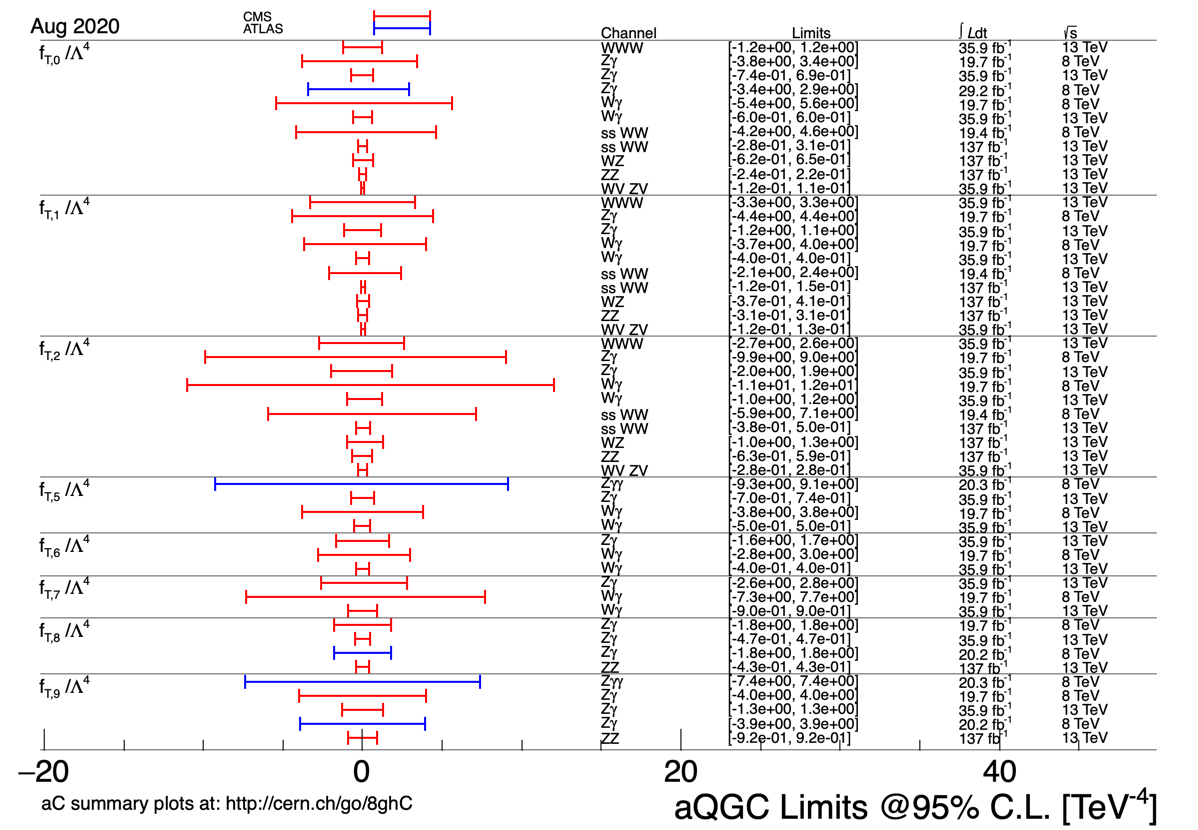
\includegraphics[width=0.80\textwidth,keepaspectratio]{figures/aQGC/aQGC_ft.png}
\caption{CMS limits on FT operatos}
\label{fig:limitFT}
\end{center}
\end{figure}

\begin{figure}[tbp]
\begin{center}
 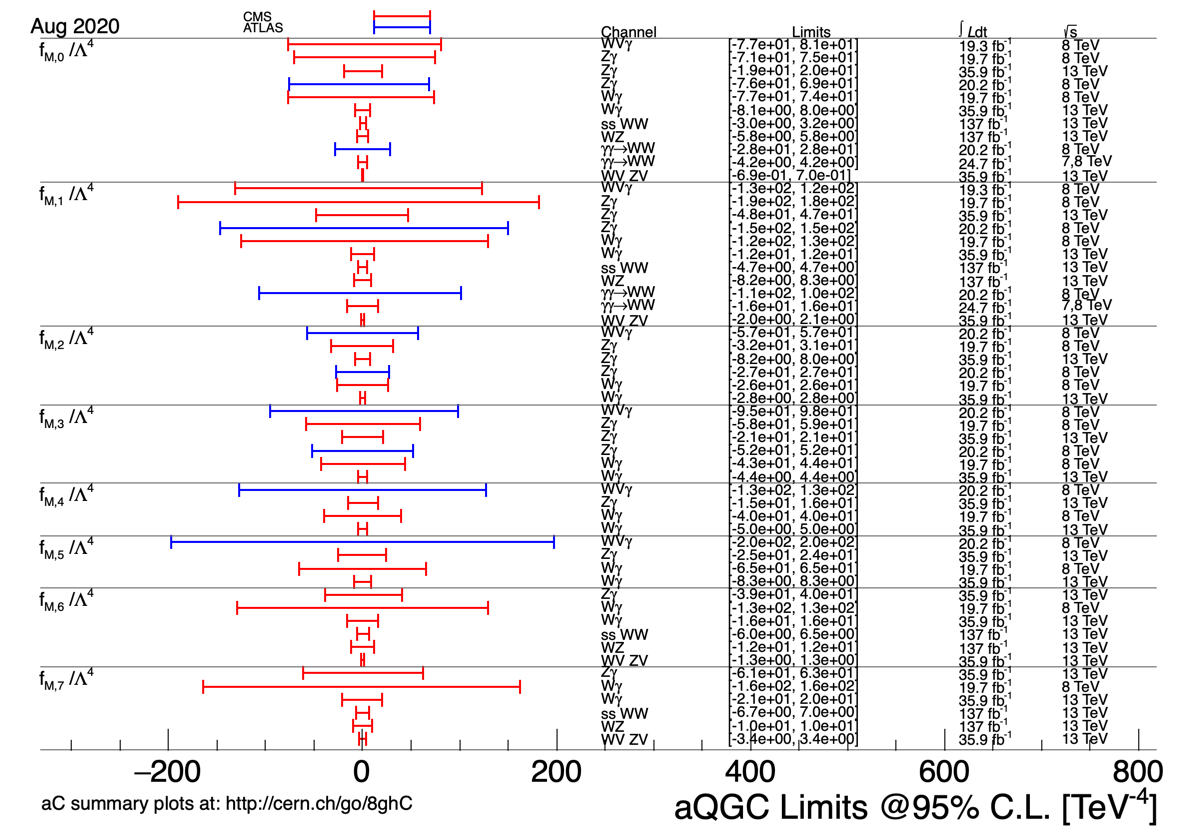
\includegraphics[width=0.80\textwidth,keepaspectratio]{figures/aQGC/aQGC_fm.png}
\caption{CMS limits on FM operatos}
\label{fig:limitFM}
\end{center}
\end{figure}

\begin{figure}[tbp]
\begin{center}
 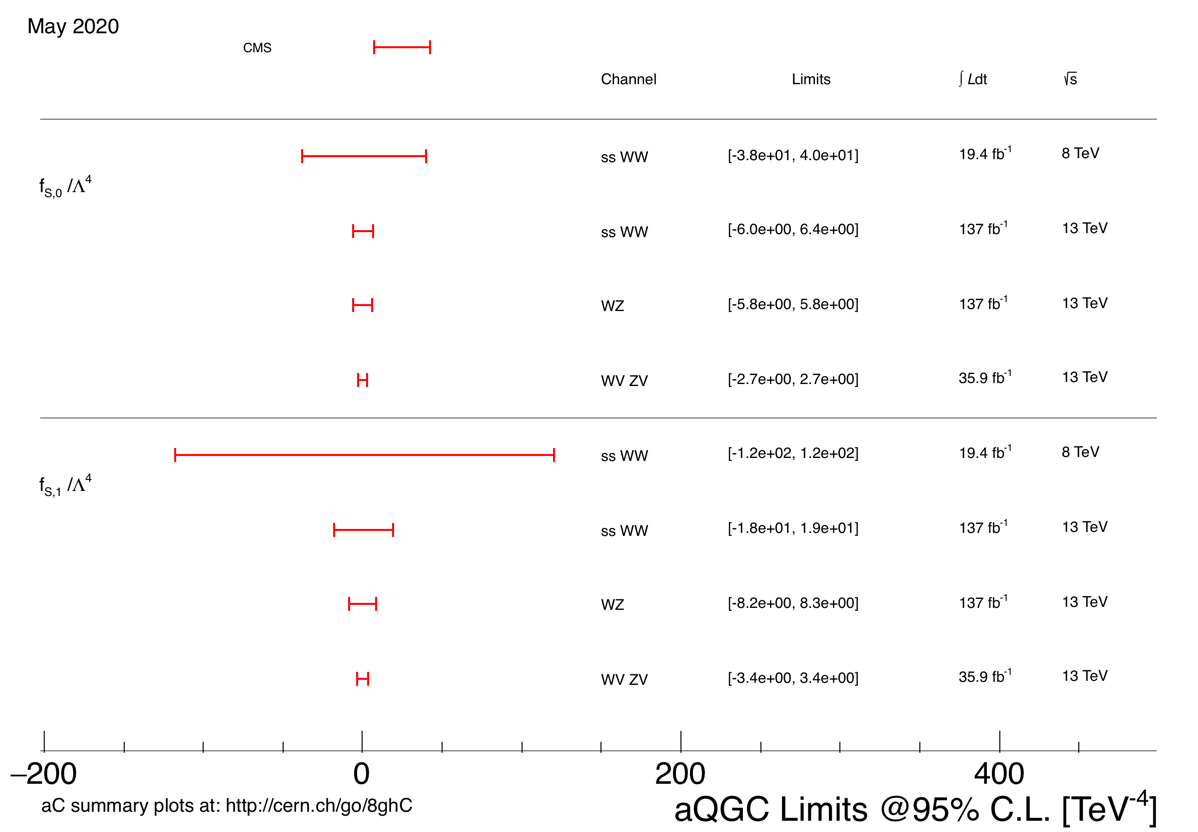
\includegraphics[width=0.80\textwidth,keepaspectratio]{figures/aQGC/aQGC_fs.png}
\caption{CMS limits on FS operatos}
\label{fig:limitFS}
\end{center}
\end{figure}

%The most stringent limits are obtained by CMS in *** channel. 

